% Appendix D: Supplementary tables and figures
\section{Supplementary material}
\label{app:supplementary}

\subsection{Kernel-weighted sector averaging}
\label{app:coeff_averaging}

\begin{table}[t]
  \centering
  \caption{Kernel-weighted sector averaging across kernel scale $\ell$ at final cutoff $N=10000$. As $\ell$ increases, unobserved-sector mixing shifts aggregate toy coefficients away from the pure $x_0$ basin values.}
  \label{tab:effective_coefficients}
  \begin{tabular}{lccccc}
    \toprule
    $\ell$ & Lambda\_Eff & G\_Eff & Q\_Fluctuation & Reheating\_Temp & Interpretation \\
    \midrule
    0.1 & 2.0000 & 0.7000 & 0.1000 & 200.0000 & Near-pure $x_0$ basin \\
    0.25 & 2.0000 & 0.7000 & 0.1000 & 200.0000 & Near-pure $x_0$ basin \\
    0.5 & 1.9817 & 0.7089 & 0.1072 & 198.1747 & Moderate mixing \\
    1.0 & 1.6781 & 0.8499 & 0.2381 & 167.8119 & Strong unobserved-sector mixing \\
    2.0 & 1.4432 & 0.9497 & 0.3497 & 144.2906 & Strong unobserved-sector mixing \\
    \bottomrule
  \end{tabular}
\end{table}


\begin{figure}[t]
  \centering
  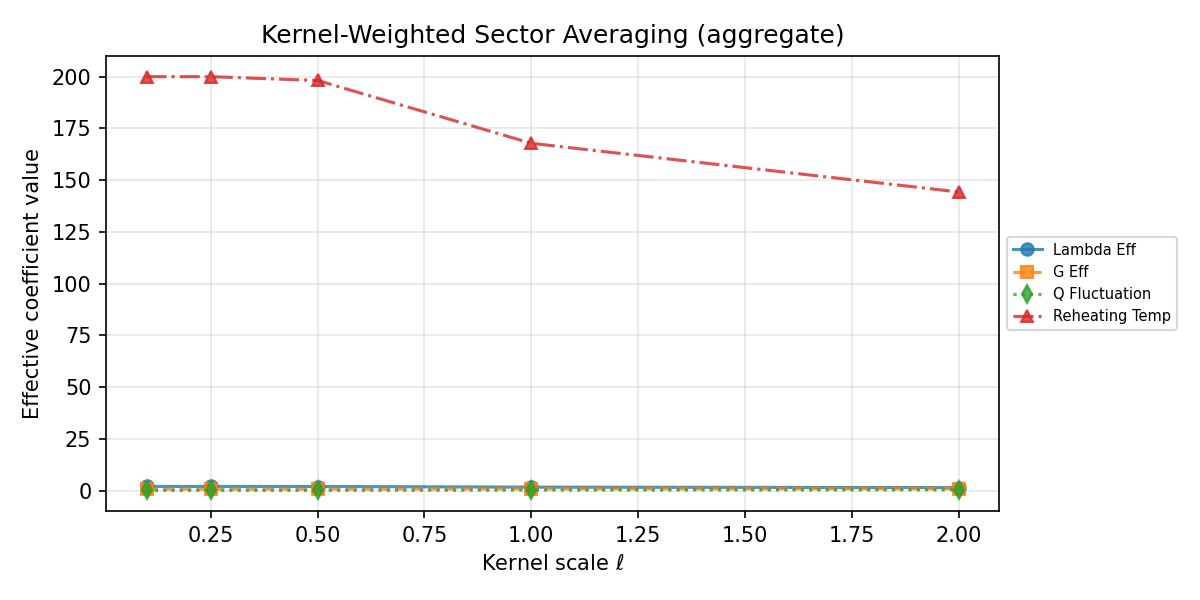
\includegraphics[width=\columnwidth]{figures/fig_06_effective_coefficient_flow.png}
  \caption{Kernel-weighted sector averaging under unobserved-sector mixing.
  As $\ell$ increases, aggregate parameters interpolate between the
  $x_0$ basin values and the global average.}
  \label{fig:coeff_flow}
\end{figure}

\subsection{Full ell sensitivity table}
\label{app:ell_sensitivity_full}

\begin{table*}[t]
  \centering
  \caption{Ell sensitivity: ISR (Gaussian kernel) stability metrics across kernel scale $\ell$ (non-degenerate regime, $\ell \ge 0.48$). The physically meaningful regime begins at $\ell \approx 0.5$, where $N_{\rm eff}$ exceeds $\sim 30\%$ of $N$. Small-$\ell$ and boundary values are diagnostic artifacts reported in Appendix~\ref{app:degenerate}. The baseline global-census KL is $3.58\times10^{-4}$.}
  \label{tab:ell_sensitivity}
  \small
  \begin{tabular}{lcccccc}
    \toprule
    $\ell$ & $N_{\rm eff}$ & KL drift & Wasserstein & Basin exc. rate & $\Lambda_{\rm eff}$ & Conv. rate \\
    \midrule
    0.48 & 3629 & $1.8\times10^{-6}$ & $2.4\times10^{-4}$ & 0.00 & 1.986 & $-1.22$ \\
    0.71 & 4793 & $4.3\times10^{-5}$ & $2.9\times10^{-3}$ & 0.00 & 1.868 & $-1.07$ \\
    1.00 & 7176 & $1.3\times10^{-4}$ & $6.6\times10^{-3}$ & 0.01 & 1.662 & $-0.93$ \\
    1.51 & 8841 & $1.9\times10^{-4}$ & $8.1\times10^{-3}$ & 0.27 & 1.511 & $-0.87$ \\
    2.20 & 9563 & $2.3\times10^{-4}$ & $8.6\times10^{-3}$ & 0.59 & 1.427 & $-0.91$ \\
    3.21 & 9860 & $2.7\times10^{-4}$ & $8.9\times10^{-3}$ & 0.61 & 1.384 & $-0.95$ \\
    10.00 & 9998 & $3.4\times10^{-4}$ & $9.2\times10^{-3}$ & 0.67 & 1.347 & $-0.98$ \\
    \bottomrule
  \end{tabular}
\end{table*}


\begin{figure}[t]
  \centering
  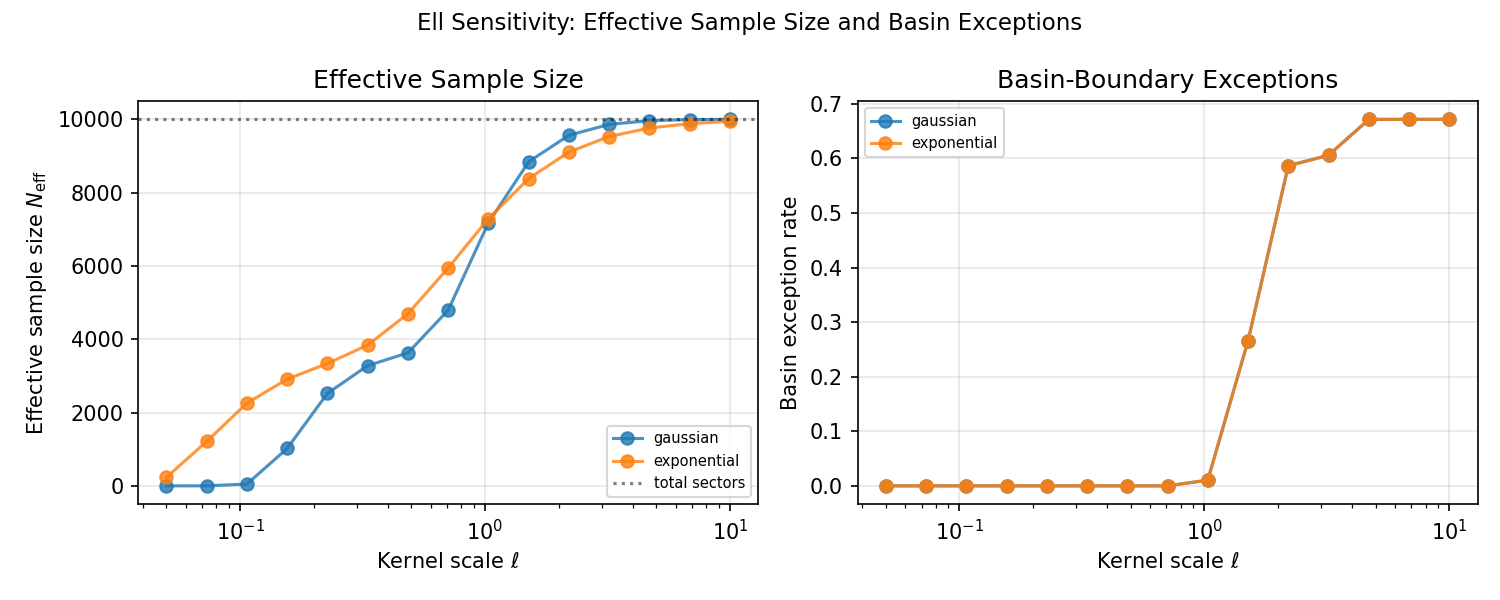
\includegraphics[width=\columnwidth]{figures/fig_12_ell_sensitivity_neff.png}
  \caption{Effective sample size $N_{\rm eff}$ and basin exception rate
  vs.\ $\ell$. The sweet spot lies where $N_{\rm eff}$ is large enough
  for statistical power but basin exceptions remain below 30\%.}
  \label{fig:ell_sensitivity_neff}
\end{figure}

\subsection{Degenerate small-$\ell$ behavior}
\label{app:degenerate}

When the kernel scale $\ell$ is much smaller than the inter-vacuum spacing
($\ell \lesssim 0.25$), the Gaussian kernel assigns non-negligible weight only
to sectors in the $x_0$ basin.
The effective sample size drops to $N_{\rm eff} \ll N$, and the ISR
distribution is effectively a delta function on the $x_0$ vacuum.
KL divergence between successive cutoffs vanishes trivially
($<10^{-25}$ at $\ell=0.05$) because there is no distribution to shift.

These values are reported separately here because they are diagnostic
artifacts, not evidence of physical stability.
Including them alongside non-degenerate results would misleadingly inflate
the apparent improvement ratio.

Tables~\ref{tab:degenerate_ell_sensitivity}~and~\ref{tab:degenerate_sigma_ell}
show the degenerate and boundary rows.

\begin{table*}[htbp!]
  \centering
  \caption{Degenerate and boundary rows from the ell sensitivity scan
  (Gaussian kernel). Rows with $\ell \lesssim 0.25$ are degenerate:
  $N_{\rm eff} \ll N$, producing trivially vanishing KL drift.
  The $\ell = 0.23$ row ($N_{\rm eff}/N = 0.25$) is a boundary case
  that narrowly fails the $N_{\rm eff}/N \ge 0.3$ threshold.}
  \label{tab:degenerate_ell_sensitivity}
  \small
  \begin{tabular}{lcccccc}
    \toprule
    $\ell$ & $N_{\rm eff}$ & KL drift & Wasserstein & Basin exc. rate & $\Lambda_{\rm eff}$ & Conv. rate \\
    \midrule
    0.05 & 1.0 & $<10^{-25}$ & $<10^{-125}$ & 0.00 & 2.000 & --- \\
    0.10 & 49.6 & $<10^{-29}$ & $<10^{-29}$ & 0.00 & 2.000 & --- \\
    0.23 & 2523 & $2.0\times10^{-10}$ & $1.6\times10^{-9}$ & 0.00 & 2.000 & $-0.07$ \\
    \bottomrule
  \end{tabular}
\end{table*}

\begin{table*}[htbp!]
  \centering
  \caption{Full sigma--ell boundary grid including degenerate small-$\ell$
  columns. Values at $\ell=0.10$ and $\ell=0.25$ are diagnostic artifacts:
  the narrow kernel forces $N_{\rm eff} \ll N$, producing trivially large
  improvement ratios.}
  \label{tab:degenerate_sigma_ell}
  \small
  \begin{tabular}{lccccc}
    \toprule
    $\sigma$ $\backslash$ $\ell$ & 0.10 & 0.25 & 0.50 & 1.00 & 2.00 \\
    \midrule
    0.5 & $2.0\times10^{21}$ & $5.6\times10^{6}$ & 68.5 & 3.12 & 1.28 \\
    1.0 & $9.6\times10^{20}$ & $2.9\times10^{5}$ & 142.5 & 5.97 & 1.86 \\
    1.5 & $1.1\times10^{21}$ & $4.1\times10^{5}$ & 240.0 & 5.38 & 2.35 \\
    2.0 & $9.2\times10^{20}$ & $2.1\times10^{5}$ & 103.1 & 7.68 & 4.40 \\
    3.0 & --- & $9.5\times10^{5}$ & 58.5 & 6.27 & 2.46 \\
    \bottomrule
  \end{tabular}
\end{table*}
